\section{Simulation}\label{sec:simulation}

Die Simulation wurde mit Hilfe von Matlab und Simulink durchgeführt.
Sie verfügt über die bereits besprochenen Attribute $c_w$-Wert, Anströmfläche $A$ und die Masse $m_S$. Weiterhin kann eine Absprunggeschwindigkeit $v_0$ und Abprunghöhe $h_0$ angegeben werden.

Die Funktion für $a_S$ (Formel~\ref{f:a_s}) wurde als Matlabfunktion (Listing~\ref{m:beschleunigung}) umgesetzt.
Eine weitere Matlabfunktion (Listing~\ref{m:c}) berechnet die Schallgeschwindigkeit in Abhängigkeit von der aktuellen Temperatur in Kelvin.

\lstinputlisting[caption={Matlabfunktion Beschleunigung},label=m:beschleunigung]{includes/beschleunigung.m}

\lstinputlisting[caption={Matlabfunktion Schallgeschwindigkeit},label=m:c]{includes/c.m}

Bei Erreichen der Höhe $0m$ wird die Simulation gestoppt.

Die Werte für Höhe, Geschwindigkeit, Beschleunigung und Schallgeschwindigkeit werden zur Analyse und Ausgabe in die aktuelle Workspace weitergegeben.

\begin{figure}[h]
  \centering
  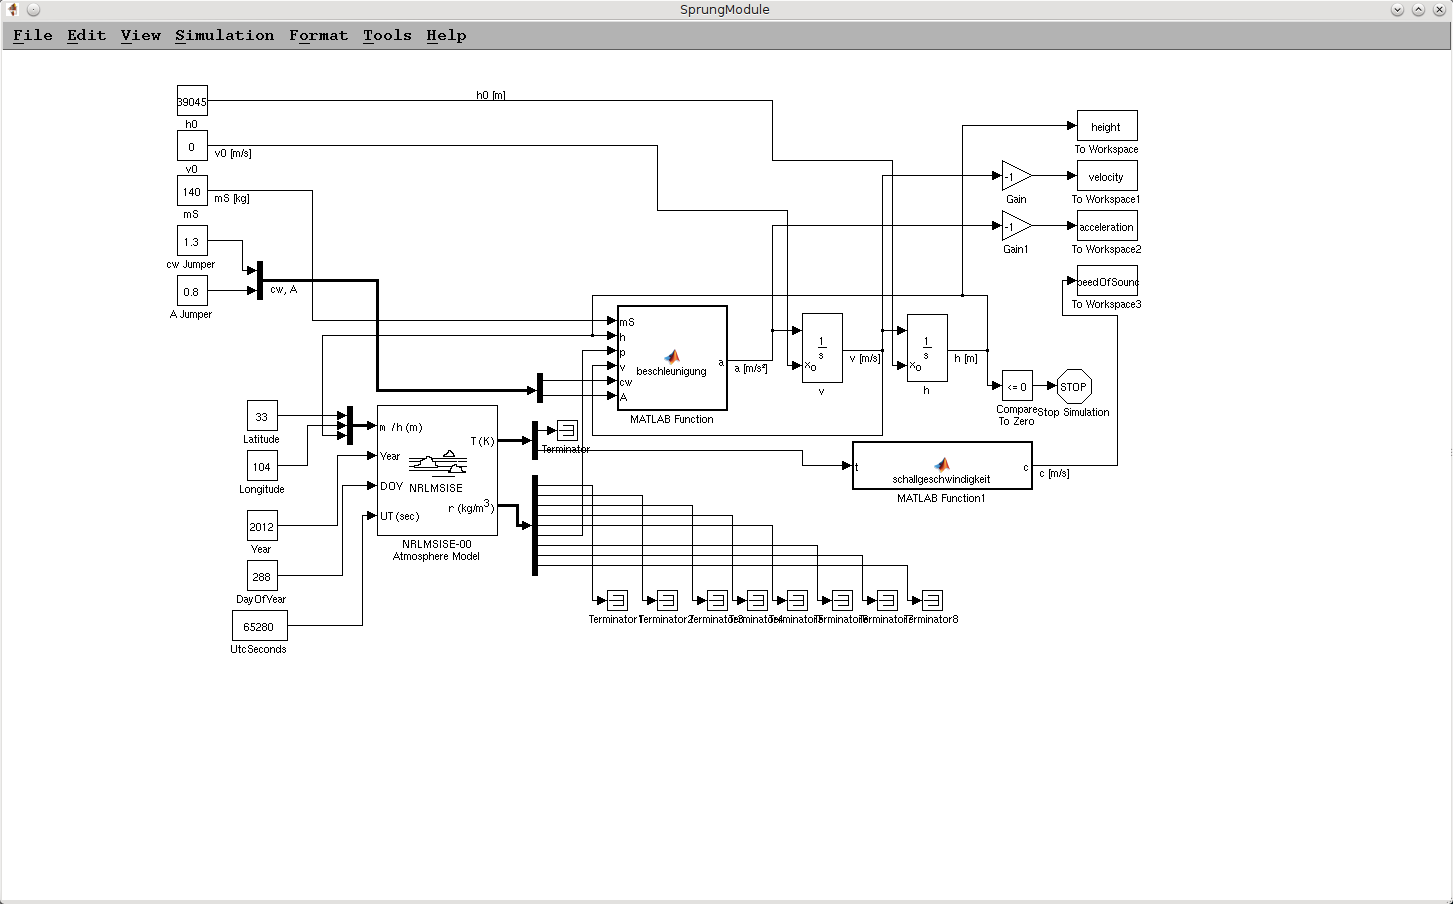
\includegraphics[width=1\textwidth]{simulink}
  \caption{Aufbau der Simulation}
  \label{fig:simulink}
\end{figure}

